\documentclass[conference]{IEEEtran}
\IEEEoverridecommandlockouts

\usepackage{amsmath,amssymb,amsfonts}
\usepackage{algorithmic}
\usepackage{graphicx}
\usepackage{textcomp}
\usepackage{xcolor}
\usepackage[style=numeric]{biblatex}

\addbibresource{references.bib}

\begin{document}

\title{Building a Fast Migration System for WireGuard}

\author{
\IEEEauthorblockN{Sina Kamali}
\textit{University of Waterloo}\\
\textit{sinakamali@uwaterloo.ca}
}

\maketitle

\section{Introduction}
WireGuard \parencite[]{Donenfeld2017} is a new tunneling protocol that operates at layer 3 by establishing a Linux virtual network interface. WireGuard provides a fully functioning tunneling system, but it makes an important assumption. WireGuard assumes that peers have a way of exchanging keys. In this work we assume that the broker is in charge of exchanging keys between clients and proxies.

There is not a established way to fast migrate a WireGuard proxy server to another already running proxy server. For a migration system to classify as a fast migration, we require two important factors:

\begin{enumerate}
    \item It should not interfere with other peers that are already connected to the destination proxy.
    \item It should have a low down time for the user.
    \item It should have a low performance cost for the system.
\end{enumerate}

To this end, we designed a novel approach to migrate WireGuard proxies, which will be detailed in full in the following sections.

\section{Design}
To support a fast migration scheme, we create a proxy and client. The proxy connects the client to a NAT server which communicates with the internet on behalf of the client. An overview of this design can be seen in \ref*{fig:odesign}.

\begin{figure}[h]
    \centering
    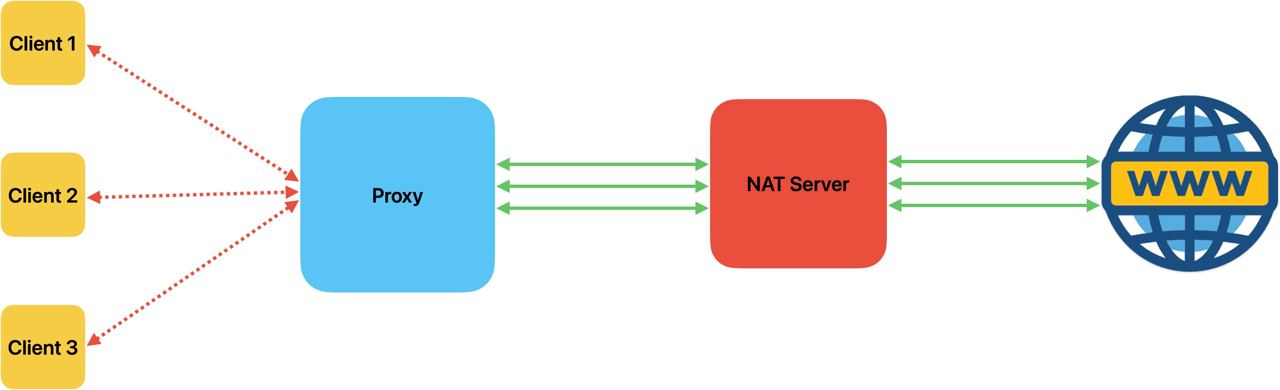
\includegraphics[scale=0.19]{fig1.jpeg}
    \caption{Hierarchical keys}
    \label{fig:odesign}
\end{figure}

\subsection{Designing the Client}
The fast migration client has a few differences from a 

\printbibliography

\end{document}
